\chapter{Giới thiệu}
\label{sec:gioithieu}


Chương này nhằm giới thiệu về bài toán sẽ được giải quyết trong luận văn và các khái niệm liên quan. Đầu chương sẽ trình bày về kỹ thuật dịch ngược, các ứng dụng của nó và những khó khăn trong quá trình dịch ngược. Phần tiếp theo nêu bài toán đặt ra và các thách thức khi giải quyết bài toán. Phần cuối cùng sẽ tóm tắt cấu trúc của luận văn.

\section{Kỹ thuật dịch ngược và ứng dụng}
Trong khi kỹ thuật dịch phổ biến hiện nay là dịch từ mã viết bằng ngôn ngữ cấp cao xuống mã ngôn ngữ cấp thấp hơn, kỹ thuật dịch ngược thực hiện dịch từ mã ngôn ngữ cấp thấp lên mã ngôn ngữ cấp cao hơn. Kỹ thuật dịch ngược được sử dụng rất nhiều để hỗ trợ trong quá trình phát triển phần mềm:

\begin{itemize}
	\item Vì một lý do nào đó, mã nguồn của một phần mềm bị mất đi. Để tiếp tục phát triển hoặc bảo trì phần mềm đó, cần phải khôi phục lại mã nguồn. Nếu viết lại một chương trình mới hoàn toàn từ các tài liệu sẵn có sẽ rất mất thời gian và không đảm bảo sẽ tương đương được phần mềm cũ. Vì vậy một giải pháp phổ biến hiện nay là dựa vào file thực thi dịch ngược lại và hiệu chỉnh để có được mã nguồn mới hoàn chỉnh.
	\item Các phần mềm độc hại như virus, malware thường sẽ giấu kín mã nguồn. Kỹ thuật dịch ngược giúp sinh ra mã nguồn của chúng, qua đó, việc tìm ra phương pháp giải trừ dễ dàng hơn.
	\item Một số chương trình được viết để chạy trên các chip đã lỗi thời, như chip 8051, sẽ ngừng sản xuất trong tương lai gần, cần phải được chuyển đổi để chạy được trên những chip hiện đại đang được sản xuất. Một trong những giải pháp để giải quyết vấn đề này là dùng trình dịch ngược để chuyển chương trình viết trên chip lỗi thời sang ngôn ngữ cấp cao, sau đó dùng trình biên dịch để dịch thành mã của chip thay thế.
	
	\begin{figure}[h]
		\centering
		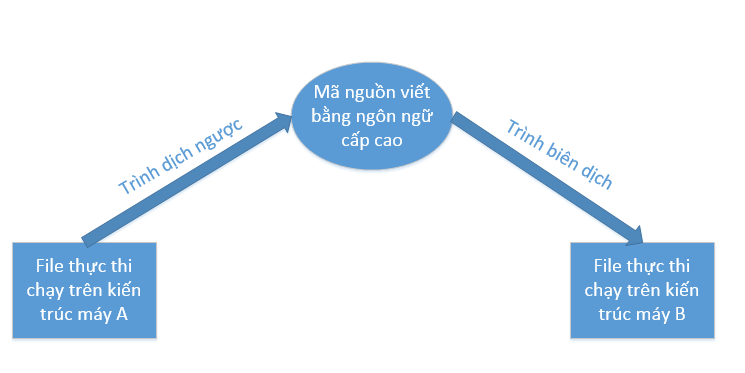
\includegraphics{fig12.png}
		\caption{Một ứng dụng của trình dịch ngược: chuyển đổi mã nguồn giữa các kiến trúc máy khác nhau}
	\end{figure}
	\item Phần mềm viết bằng ngôn ngữ A cần phải chuyển đổi sang ngôn ngữ B để tiếp tục bảo trì và phát triển. Ngôn ngữ A có thể là một ngôn ngữ đã ra đời từ rất lâu (ví dụ: COBOL, Basic...), hiện nay không còn người hiểu biết về ngôn ngữ đó để lập trình phần mềm. Vì vậy, cần phải chuyển đổi phần mềm sang một ngôn ngữ khác mới hơn, có nhân lực để viết tiếp (ví dụ: Java, C\#...). Quá trình này cũng được xem là dịch ngược, vì thường ngôn ngữ A ra đời trước sẽ có mức độ trừu tượng thấp hơn là các ngôn ngữ B được phát triển sau này.
\end{itemize}

Một trong những thách thức khó nhất của kỹ thuật dịch ngược là khôi phục thông tin. Do ở các ngôn ngữ cấp thấp không có phương tiện để lưu trữ một số thông tin cần thiết ở ngôn ngữ cấp cao, nên những thông tin đó sẽ bị mất đi trong quá trình dịch xuôi hoặc lập trình bằng ngôn ngữ cấp thấp. Một số thông tin cần khôi phục là:
\begin{itemize}
	\item Kiểu dữ liệu của biến: Đối với các chương trình viết bằng ngôn ngữ cấp cao, kiểu dữ liệu của biến có thể xem như một ràng buộc khi gán giá trị cho biến và sử dụng biến. Ví dụ khi ta khai báo một biến có kiểu dữ liệu là integer, thì ta phải gán cho biến các giá trị là số nguyên (1, 2,...) và sử dụng biến trong các phép toán có toán tử là số nguyên. Nếu ta gán cho biến một giá trị khác số nguyên (số thực, chuỗi, boolean...) hoặc sử dụng biến trong các phép toán không chấp nhận toán tử là số nguyên thì trình biên dịch sẽ phát hiện lỗi ngay ở giai đoạn đầu. Tuy nhiên, đối với một số mã máy, kiểu dữ liệu không cần thiết và sẽ được loại bỏ trong quá trình biên dịch. Khi dịch ngược, nếu không khôi phục được kiểu dữ liệu thì sẽ không đủ thông tin để xây dựng mã đầu ra.
	
	\item Tên của biến: Ở ngôn ngữ cấp cao, tên biến mang ngữ nghĩa là công dụng của biến đó, và được dùng để truy xuất giá trị của biến. Còn ở ngôn ngữ cấp thấp, dữ liệu sẽ được lưu vào các thanh ghi có sẵn hoặc vùng nhớ được truy xuất bằng địa chỉ trực tiếp, vì vậy việc tên biến ở cấp độ này là không cần thiết và sẽ bị loại bỏ. Nếu trình dịch ngược không giữ được tên biến của chương trình gốc thì rất khó để phát triển và bảo trì. Giải pháp hiện nay của các trình dịch ngược là sinh ra tên biến tự động, sau đó dựa vào các tài liệu sẵn có để chỉnh sửa tên biến bằng tay ở chương trình đầu ra.
	
	\item Phân biệt giữa dữ liệu và mã điều khiển: Đặc điểm của một số mã máy (trừ mã	máy chạy trên máy ảo) là dữ liệu và các câu lệnh điều khiển có cùng một định dạng mã nhị phân và được lưu trong cùng một vùng nhớ. Vì vậy, khi dịch ngược từ mã máy lên cần phải phân biệt được phần nào của vùng nhớ là lưu các dữ liệu và phần nào là câu lệnh của chương trình.
\end{itemize}

Từ khái niệm của kỹ thuật dịch ngược, ta thấy có nhiều mức độ dịch ngược, tương ứng với những bài toán khác nhau cần giải quyết. Nếu lấy đầu ra của quá trình dịch ngược là một chương trình viết bằng ngôn ngữ cấp cao, thì đầu vào của nó có thể là: mã nhị phân, mã assembly hoặc mã của một ngôn ngữ lập trình cấp cao khác cần chuyển đổi. Tùy vào mức độ trừu tượng của ngôn ngữ đầu vào, các thông tin bị mất ở mã đầu vào sẽ khác nhau. Với mã máy thì tất cả các thông tin nêu trên đều không còn. Với mã assembly, tên biến vẫn xuất hiện trong chương trình vì một số assembler cho phép có các câu lệnh khai báo biến ở mã assembly. Còn với mã ngôn ngữ cấp cao thì gần như tất cả thông tin đều có ở chương trình gốc, và vấn đề cần giải quyết là tìm ra các cấu trúc tương đương ở ngôn ngữ đích.

\section{Bài toán đặt ra}
\label{sec:problem}
Như đã trình bày ở trên, kiểu dữ liệu là một thông tin quan trọng không xuất hiện ở mã cấp thấp nhưng cần phải có để xây dựng mã đầu ra của trình dịch ngược. Vì vậy, bài toán suy luận kiểu là một thách thức cấp bách cần phải giải quyết trong kỹ thuật dịch ngược. Hiện nay, các giải thuật cho vấn đề này đã tương đối đầy đủ, đưa ra kết quả kiểu dữ liệu chấp nhận được. Tuy nhiên, có vấn đề chưa được giải quyết thấu đáo là ở một số kiến trúc máy, người lập trình có thể vừa truy xuất một vùng nhớ lớn, vừa truy xuất một vùng nhớ nhỏ hơn thuộc vùng nhớ lớn đó, đồng thời có thể đặt tên các vùng nhớ. Vì việc thay đổi giá trị một vùng nhớ nhỏ cũng sẽ làm thay đổi giá trị của vùng nhớ lớn hơn, nên không thể xem vùng nhớ nhỏ như một biến độc lập, mà cần phải gom nhóm các biến đại diện cho vùng nhớ nhỏ và vùng nhớ lớn thành một cấu trúc dữ liệu phù hợp ở ngôn ngữ cấp cao. \\

Một kiến trúc máy có những tính chất trên là 8051. Như trong ví dụ \ref{list:8051exam}, có 2 biến được khai báo là \textit{OPTIONS} với giá trị là \textbf{38H}, và \textit{TESTSUPS} đại diện cho bit thứ nhất của thanh ghi \textit{ACC}. Ở đoạn mã thực thi bên dưới, thanh ghi \textit{ACC} được gán cho giá trị ở vùng nhớ có địa chỉ là giá trị của biến \textit{OPTIONS} (câu lệnh số 1) và sau đó giá trị của \textit{TESTUPS} được chuyển thành 1, nghĩa là bit đầu tiên của thanh ghi \textit{ACC} bật lên. Qua thấy được thanh ghi \textit{ACC} chỉ là trung gian, và thực chất \textit{TESTUPS} đại diện cho bit đầu tiên của vùng nhớ quy định bởi biến \textit{OPTIONS}. Việc sử dụng này đưa đến kết luận là biến \textit{OPTIONS} và \textit{TESTUPS} là cùng một bộ biến vì đều truy xuất đến toàn bộ hoặc một phần vùng nhớ có địa chỉ là \textbf{38H}.

\begin{lstlisting}[caption={Một đoạn mã 8051},label={list:8051exam}]
#DEFINE OPTIONS, #38H
#DEFINE TESTSUPS ACC.1
public AA
AA:
	MOV A, OPTIONS #1
	SETB TESTUPS #2
\end{lstlisting}

Trong bộ biến này, \textit{OPTIONS} được gọi là \textbf{biến byte}, vì nó truy xuất đến vùng nhớ có độ lớn là 1 byte. Còn các biến truy xuất đến một bit nào đó của vùng nhớ như \textit{TESTSUPS} sẽ được gọi là \textbf{biến bit}. Thông thường, người ta luôn sử dụng các biến byte - biến bit này theo bộ và việc sử dụng các bộ biến này phải tuân thủ nguyên tắc sau: 
\begin{itemize}
	\item Chỉ khi thanh ghi \textit{ACC} đang mang giá trị của vùng nhớ có địa chỉ quy định bởi biến byte, thì các biến bit cùng bộ mới được sử dụng.
	\item Mỗi biến bit chỉ thuộc một bộ duy nhất. Nói cách khác, nếu mỗi thời điểm sử dụng biến bit, thanh ghi \textit{ACC} đang mang giá trị của nhưng vùng nhớ khác nhau, thì việc sử dụng này đã vi phạm nguyên tắc.
	\item Tại mỗi vị trí bit của một bộ biến chỉ có một biến bit duy nhất tồn tại. Một ví dụ vi phạm nguyên tắc này là ở đoạn mã \ref{list:illegalexam}. Khi thanh ghi \textit{ACC} đang mang giá trị vùng nhớ quy định bởi \textit{OPTIONS}, có hai biến bit cùng truy xuất đến bit đầu tiên của vùng nhớ được sử dụng là \textit{TESTSUPS} và \textit{TESTSUPS1}. Như vậy, ta không thể chọn được biến bit nào sẽ đại diện cho bit đầu tiên của vùng nhớ giữa hai biến trên.
	\begin{lstlisting}[caption={Một ví dụ vi phạm nguyên tắc sử dụng bộ biến},label={list:illegalexam}]
	#DEFINE OPTIONS #38H 
	#DEFINE TESTSUPS ACC.1
	#DEFINE TESTSUPS1 ACC.1
	
	public AA
	AA:
	MOV A, OPTIONS
	SETB TESTSUPS
	CLR TESTSUPS1
	\end{lstlisting}
\end{itemize}
Vì 8051 đáp ứng đầy đủ các yêu cầu về một kiến trúc máy cho phép truy xuất vùng nhớ ở nhiều cấp độ và cho phép đặt tên biến cho vùng nhớ, nên các phân tích sau này của luận văn sẽ chủ yếu dựa vào các đoạn mã của 8051. Tuy nhiên, các nghiên cứu này hoàn toàn có thể áp dụng cho các kiến trúc máy có tính chất tương tự như vậy. Về sau trong luận văn này, khi đề cập đến nguyên tắc sử dụng bộ biến, nghĩa là đang nói đến các nguyên tắc nêu trên. \\

Union là một cấu trúc dữ liệu có nhiều thành phần với những kiểu dữ liệu khác nhau, nhưng cùng chia sẻ một vùng nhớ. Trong ví dụ \ref{list:uniondecl}, hai thành phần của union \textit{ci} là ký tự \textit{c} và số nguyên \textit{i} đều có vùng nhớ giống nhau. Khi thay đổi một thành phần như ở câu lệnh số 3, thành phần còn lại của union cũng thay đổi theo. Giá trị \textit{ci.i} được xuất ra ở câu lệnh số 2 là \textbf{0} (giá trị mặc định của một số nguyên chưa khai báo), còn ở câu lệnh số 4 là \textbf{97}. Như vậy, tính chất này của union là tương tự với tính chất truy xuất vùng nhớ đã nêu ở trên của một số kiến trúc máy.\\
\begin{lstlisting}[caption={Một đoạn khai báo union},label={list:uniondecl},language=c++]
union {char c; int i;} ci;
cout << i;
ci.c = 'a';
cout << i;
\end{lstlisting}

\textit{Tóm lại, luận văn sẽ giải quyết vấn đề gom nhóm biến truy xuất toàn bộ một vùng nhớ và những biến truy xuất một phần vùng nhớ đó, đưa chúng về dưới dạng cấu trúc dữ liệu union ở ngôn ngữ cấp cao.}\\

Để giải quyết vấn đề này, có hai hướng tiếp cận được đề ra trong luận văn. Đó là:
\begin{itemize}
	\item Dựa trên một số thông tin trong phần chú thích của người lập trình viên. Trong quá trình lập trình, để biết được các biến nào cùng một bộ với nhau, người lập trình phải có chú thích ở phần khai báo của các biến đó. Giải pháp đề ra là đưa ra một mẫu quy định các chú thích này, yêu cầu người lập trình sửa chữa chú thích của mình theo mẫu đó, sau đó dùng parser rút trích thông tin từ chú thích để tìm ra các bộ biến và kiểm tra việc sử dụng biến bên dưới (Kiểm tra kiểu - Type checking).
	\item Dựa vào quá trình sử dụng các biến trong chương trình. Việc chú thích là không bắt buộc với lập trình viên, nên một số đoạn mã có thể bị thiếu chú thích hoặc chú thích không đầy đủ. Cách giải quyết khả thi là xem xét quá trình sử dụng các biến, phân tích luồng đi của dữ liệu và tìm ra được các union phù hợp (Suy luận kiểu - Type reference).
\end{itemize}
\begin{figure}
	\centering
	
\includegraphics[width=0.7\linewidth]{image/main}
	\caption{Các hướng tiếp cận được trình bày trong luận văn}
	\label{fig:main}
\end{figure}
\section{Cấu trúc luận văn}

Luận văn gồm có 6 chương. Chương tiếp theo sẽ trình bày về các kiến thức nền tảng, cũng như một số nghiên cứu liên quan đến kỹ thuật dịch ngược. Ngoài ra, chương này cũng chỉ rõ kiến trúc của trình dịch ngược Boomerang, trình dịch ngược được dùng để hiện thực các giải pháp của bài toán. Chương 3 giới thiệu hướng tiếp cận đầu tiên của bài toán là rút trích thông tin từ các chú thích của người lập trình. Chương 4 sẽ làm rõ hướng tiếp cận tiếp theo là dựa vào cách sử dụng biến trong đoạn mã đầu vào. Chương 5 nêu ra một số thiết lập cần thiết trên trình dịch ngược Boomerang để kiểm tra kết quả của hai hướng tiếp cận trên, cách thiết lập các mẫu thử (testcase) và kết quả chạy thử. Chương 6 kết luận về kết quả đạt được của luận văn và đề ra các hướng nghiên cứu tiếp theo.
	
\begin{comment}
Như đã đề cập ở phần trên, mục tiêu của luận văn là nghiên cứu về trình dịch ngược từ mã assembly lên mã cấp cao, các bài toán cần phải giải quyết và hiện thực giải pháp. Vì mã assembly cho kiến trúc máy khác nhau có những đặc điểm khác nhau, và đi cùng với đó là những vấn đề khác nhau cần giải quyết, nên giới hạn của luận văn sẽ là trình dịch ngược từ mã assembly 8051. Việc chọn kiến trúc máy 8051 là do 2 nguyên nhân sau:
\begin{itemize}
	\item Chip 8051 đã xuất hiện trên thị trường từ lâu, hiện tại sắp không còn được sản xuất. Tuy nhiên, vẫn còn nhiều hệ thống được chạy trên đây và cần phải chuyển đổi chúng sang một kiến trúc máy khác hiện đại hơn. Như vậy, nhu cầu đặt ra là có thực.
	\item Chip 8051 có một số đặc điểm khác biệt so với các con chip khác trên thị trường. Vì vậy việc dịch ngược từ mã 8051 sẽ gặp nhiều khó khăn hơn, vấn đề phải giải quyết phức tạp hơn. 
\end{itemize}

Các đặc điểm khác biệt của 8051 gồm có:
\begin{itemize}
	\item Trong khi hầu hết các kiến trúc máy khác sử dụng kiểu dữ liệu byte là kiểu dữ liệu nhỏ nhất, thì 8051 cho phép lập trình viên truy xuất tới mức bit trong một số thanh ghi và kèm theo đó là các câu lệnh xử lý bit. Tuy nhiên, các thanh ghi này của 8051 cũng có thể được truy xuất ở mức byte bình thường. Xem ví dụ ở đoạn mã \ref{list:list1}, câu lệnh số 1 gán giá trị ở vùng nhớ có địa chỉ 38H cho toàn bộ thanh ghi ACC, trong khi câu lệnh số 2 chỉ sử dụng biến số 1 của thanh ghi ACC.
	\begin{lstlisting}[caption={Một đoạn mã 8051 sử dụng cả biến bit và biến byte của thanh ghi ACC},label={list:list1}]
	MOV ACC, 38H #1
	SETB ACC.1 #2
	\end{lstlisting}
	\item Một số assembler của 8051 cho phép sử dụng tên biến. Biến này dùng để lưu các giá trị hằng số, hằng số này thường là địa chỉ một vùng nhớ kích thước 1 byte (trong luận văn này sẽ gọi tắt là biến byte) hoặc đại diện cho bit của thanh ghi (gọi tắt là biến bit). Khi lập trình, người ta thường sử dụng biến byte và biến bit này theo bộ, nghĩa là chỉ khi thanh ghi được load vào giá trị vùng nhớ quy định bởi biến byte, thì các biến bit cùng bộ mới được sử dụng (xem ví dụ ở đoạn mã \ref{list:list2}) (từ nay, khi luận văn sử dụng từ "nguyên tắc sử dụng bộ biến", nghĩa là đang đề cập đến nguyên tắc này).
		\begin{lstlisting}[caption={Một đoạn mã 8051 tuân theo nguyên tắc sử dụng bộ biến},label={list:list2}]
	#DEFINE OPTIONS #38H
	#DEFINE TESTSUP ACC.1
	public AA
	AA: 
	MOV ACC, OPTIONS
	JB TESTSUP, BB
	\end{lstlisting}
\end{itemize}

Từ các đặc điểm trên, ta có thể thấy bài toán lớn nhất đặt ra trong luận văn này sẽ là tìm ra được mối liên hệ giữa biến byte và biến bit trong chương trình, lấy được các bộ biến byte và biến bit đúng. Có 2 cách để biết được điều này:
\begin{itemize}
	\item Đưa ra quy định về việc khai báo biến byte và biến bit. Hiện nay, ở phần khai báo, các lập trình viên có thể khai báo các biến theo thứ tự tuỳ ý, và cũng không có quy định nào bắt buộc họ phải có phần comment chỉ rõ các biến byte và biến bit nào là cùng một bộ. Ta có thể đưa ra các mẫu khai báo cho biến byte và biến bit để trình dịch ngược có thể biết được các bộ biến bằng cách đọc theo mẫu mà không cần phân tích gì thêm. Tuy nhiên, sau khi đã xác định được các bộ biến này, cần có thêm một bước kiểm tra mã chương trình để đảm bảo rằng nguyên tắc sử dụng biến byte và biến bit được tuân thủ. Vì vậy, ta sẽ gọi giải pháp này là Kiểm tra kiểu - Type checking. Giải pháp này có ưu điểm là đơn giản, dễ hiện thực nhưng gây bất tiện cho người dùng vì phải chuyển đổi bộ mã hiện tại về theo mẫu quy định.
	\item Dựa vào phân tích luồng dữ liệu của chương trình, tìm ra được địa chỉ vùng nhớ được load vào thanh ghi tại thời điểm sử dụng biến bit và từ đó suy ra biến byte cùng bộ với biến bit đó. Giải pháp này được đặt tên là Suy luận kiểu - Type inference. Với cách làm này, không cần phải thay đổi đoạn mã gốc. Tuy nhiên cách hiện thực sẽ phức tạp hơn nhiều vì có rất nhiều cách load dữ liệu vùng nhớ vào thanh ghi như: dùng trực tiếp hằng số, dùng trực tiếp biến byte, trung gian qua một thanh ghi khác, dùng một biểu thức toán học có 2 vế... (xem ví dụ ở đoạn mã \ref{list:list3})
		\begin{lstlisting}[caption={Ví dụ một số mẫu câu lệnh load vùng nhớ vào thanh ghi trong 8051},label={list:list1}]
	MOV ACC, 38H
	MOV ACC, OPTIONS
	MOV ACC, @DPTR
	MOV ACC, OPTIONS+1
	\end{lstlisting}
\end{itemize}

Cả hai giải pháp này đều được hiện thực trong từng giai đoạn của luận văn và sẽ được trình bày trong các chương tiếp theo.

Ngoài ra, một công việc khác cần phải làm đó là giữ nguyên tên biến trong quá trình dịch ngược. Hiện tại trình dịch ngược Boomerang chỉ cho phép ta định nghĩa trước một số thanh ghi trong một kiến trúc máy, và đoạn mã đầu vào chỉ được sử dụng các thanh ghi đó, nếu sử dụng một cái tên nằm ngoài danh sách thanh ghi thì sẽ báo lỗi. Vì vậy, ta sẽ phải điều chỉnh cơ chế này, cho phép việc sử dụng tên biến khác và giữ nguyên chúng khi dịch ra đoạn mã ngôn ngữ cấp cao.

\section{Cấu trúc luận văn}
Luận văn sẽ gồm 6 chương như sau:
\begin{itemize}
	\item Chương 1: Giới thiệu về kỹ thuật dịch ngược, bài toán đặt ra trong luận văn và cấu trúc của luận văn.
	\item Chương 2: Nêu lên một số kiến thức cơ bản và các nghiên cứu liên quan đến luận văn. Đặc biệt, trong chương này sẽ trình bày một số kiến thức cơ bản về Boomerang, giúp người đọc dễ dàng hiểu các phần sau hơn.
	\item Chương 3: Trình bày giải pháp Kiểm tra kiểu - Type checking. Ngoài ra, trong chương này sẽ trình bày cơ chế cho phép đọc tên biến khác thanh ghi và lưu trữ chúng trong trình dịch ngược, vì đây là bước đầu tiên trong quá trình thực hiện các giải pháp.
	\item Chương 4: Trình bày giải pháp Suy luận kiểu - Type inference.
	\item Chương 5: Đánh giá kết quả của luận văn thông qua các mẫu thử (testcase).
	\item Chương 6: Kết luận.
\end{itemize}
\end{comment}